%Amazon


\begin{figure}[htbp]
\centering
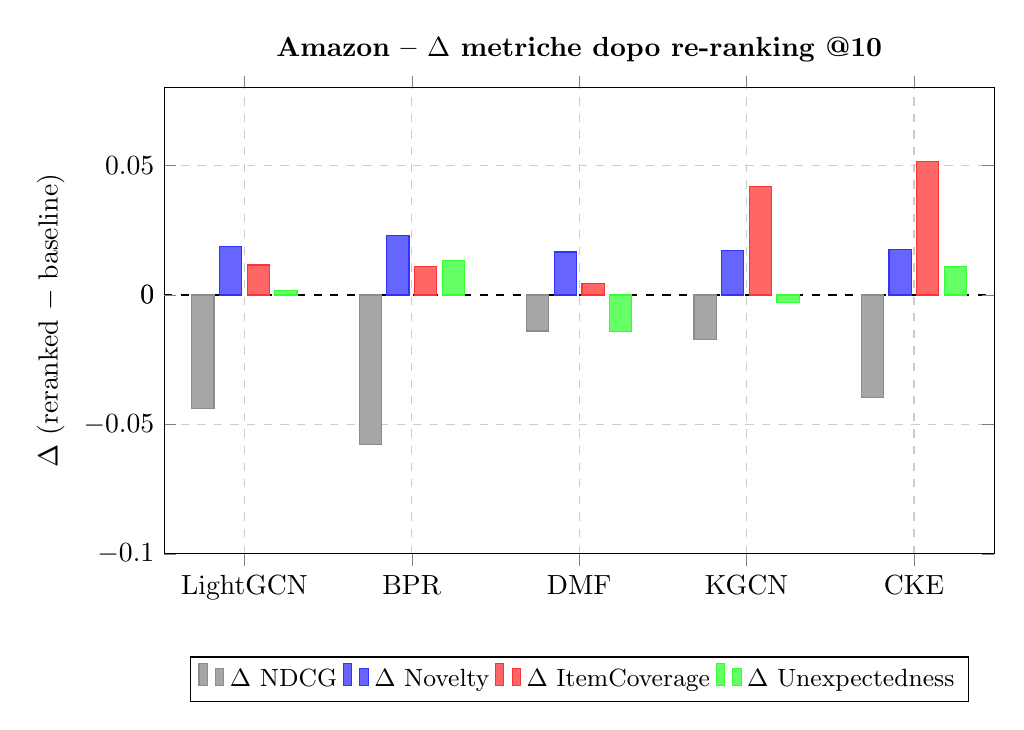
\begin{tikzpicture}
\begin{axis}[
    ybar,
    bar width=8pt,
    width=\textwidth,
    height=7.5cm,
    enlarge x limits=0.12,
    legend style={at={(0.5,-0.22)}, anchor=north, legend columns=4, font=\small},
    ylabel={$\Delta$ (reranked $-$ baseline)},
    symbolic x coords={LightGCN, BPR, DMF, KGCN, CKE},
    xtick=data,
    ymin=-0.10, ymax=0.08,
    yticklabel style={/pgf/number format/.cd, fixed, precision=3},
    title={Amazon -- $\Delta$ metriche dopo re-ranking @10},
    title style={font=\bfseries},
    grid=major,
    grid style={dashed, gray!40},
    extra y ticks={0},
    extra y tick style={grid=major, grid style={black, thick}},
]
\addplot[fill=gray!70, draw=gray!90]
    coordinates {(LightGCN,-0.0437) (BPR,-0.0578) (DMF,-0.0139) (KGCN,-0.0173) (CKE,-0.0395)};
\addplot[fill=blue!60, draw=blue!80]
    coordinates {(LightGCN,0.0188) (BPR,0.0229) (DMF,0.0166) (KGCN,0.0173) (CKE,0.0176)};
\addplot[fill=red!60, draw=red!80]
    coordinates {(LightGCN,0.0116) (BPR,0.0109) (DMF,0.0046) (KGCN,0.0420) (CKE,0.0517)};
\addplot[fill=green!60, draw=green!80]
    coordinates {(LightGCN,0.0019) (BPR,0.0132) (DMF,-0.0142) (KGCN,-0.0029) (CKE,0.0110)};
\legend{$\Delta$ NDCG, $\Delta$ Novelty, $\Delta$ ItemCoverage, $\Delta$ Unexpectedness}
\end{axis}
\end{tikzpicture}
\caption{Delta delle metriche principali dopo re-ranking (Amazon). Valori positivi
indicano miglioramento, valori negativi indicano degradazione.}
\label{fig:rq2_amazon}
\end{figure}



%MovieLens


\begin{figure}[H]
\centering
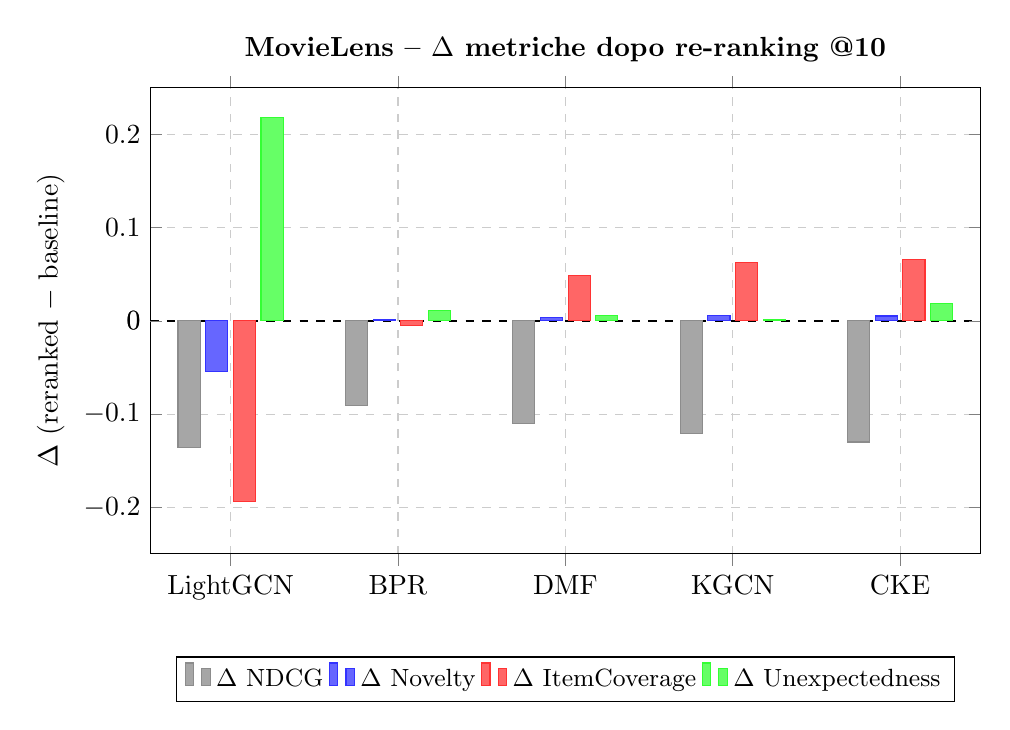
\begin{tikzpicture}
\begin{axis}[
    ybar,
    bar width=8pt,
    width=\textwidth,
    height=7.5cm,
    enlarge x limits=0.12,
    legend style={at={(0.5,-0.22)}, anchor=north, legend columns=4, font=\small},
    ylabel={$\Delta$ (reranked $-$ baseline)},
    symbolic x coords={LightGCN, BPR, DMF, KGCN, CKE},
    xtick=data,
    ymin=-0.25, ymax=0.25,
    yticklabel style={/pgf/number format/.cd, fixed, precision=3},
    title={MovieLens -- $\Delta$ metriche dopo re-ranking @10},
    title style={font=\bfseries},
    grid=major,
    grid style={dashed, gray!40},
    extra y ticks={0},
    extra y tick style={grid=major, grid style={black, thick}},
]
\addplot[fill=gray!70, draw=gray!90]
    coordinates {(LightGCN,-0.1356) (BPR,-0.0911) (DMF,-0.1102) (KGCN,-0.1205) (CKE,-0.1300)};
\addplot[fill=blue!60, draw=blue!80]
    coordinates {(LightGCN,-0.0547) (BPR,0.0019) (DMF,0.0037) (KGCN,0.0054) (CKE,0.0052)};
\addplot[fill=red!60, draw=red!80]
    coordinates {(LightGCN,-0.1937) (BPR,-0.0054) (DMF,0.0488) (KGCN,0.0626) (CKE,0.0662)};
\addplot[fill=green!60, draw=green!80]
    coordinates {(LightGCN,0.2179) (BPR,0.0115) (DMF,0.0054) (KGCN,0.0009) (CKE,0.0182)};
\legend{$\Delta$ NDCG, $\Delta$ Novelty, $\Delta$ ItemCoverage, $\Delta$ Unexpectedness}
\end{axis}
\end{tikzpicture}
\caption{Delta delle metriche principali dopo re-ranking @10 (MovieLens). Valori positivi
indicano miglioramento, valori negativi indicano degradazione.}
\label{fig:rq2_movielens}
\end{figure}